\documentclass[a4paper]{article}

\usepackage[utf8]{inputenc}
\usepackage[ngerman]{babel}
\usepackage{amsmath,amssymb}
\usepackage[german,vlined,longend]{algorithm2e}
\usepackage{graphicx}
\PassOptionsToPackage{usenames,dvipsnames,svgnames}{xcolor}  
\usepackage{tikz}
\usetikzlibrary{arrows,positioning,automata}
\usepackage{listings}

% --- math operators ---
\usepackage{mathtools}
\DeclarePairedDelimiter\set{\{}{\}} % use $\set*{1, 2, 3}$ 
\DeclarePairedDelimiter\abs{\lvert}{\rvert}
\DeclarePairedDelimiter\norm{\lVert}{\rVert}
\DeclarePairedDelimiter\ceils{\lceil}{\rceil}
\DeclarePairedDelimiter\floor{\lfloor}{\rfloor}
\DeclarePairedDelimiter\angles{\langle}{\rangle}
\def\Oh{\ensuremath{\mathcal{O}}} % big O like $\Oh(n)$
\def\oh{\ensuremath{\scriptstyle{\mathcal{O}}}} % small O
% ---

\begin{document}

\begin{small}
	\noindent
	Schubert Julian, Gruppe 4 \\
	Philipp Wahl, Gruppe 4
\end{small}
\bigskip

\begin{center}
	\LARGE Abgabe zum 1. Übungsblatt (AGT 21)
\end{center}
\smallskip

\subsection*{Aufgabe 1:}

\paragraph{a)}
\begin{tabular}{ |c | c | c | c | c | c | c |}
    \hline
    \textbf{t}  & \textbf{u}& \textbf{v}& \textbf{w}& \textbf{x}& \textbf{y}& \textbf{z} \\
    \hline
    $\infty$    & $\infty$  & $\infty$  & $\infty$  & 0         & $\infty$  & $\infty$ \\
    $\infty$    & \textbf{2}& 3         & 6         & 0         & $\infty$  & $\infty$ \\
    $\infty$    &           &\textbf{3} & 6         & 0         & 12        & $\infty$ \\
    $\infty$    &           &           & \textbf{5}& 0         & 12        & 9 \\
    9           &           &           &           & 0         & 12        &\textbf{7} \\
    \textbf{9}  &           &           &           & 0         & 10        & \\
                &           &           &           & 0         & \textbf{10}& \\
    \hline
\end{tabular}
\paragraph{b)}

\begin{figure}[htb]
\centering
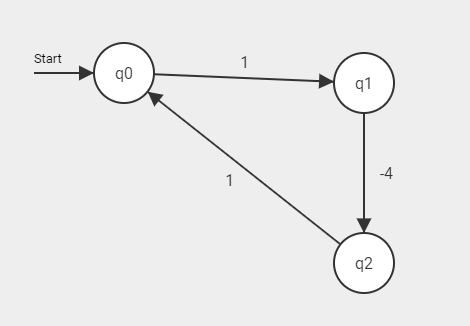
\includegraphics[width=0.9\linewidth]{01.png}
\label{fig:name}
\end{figure}

\begin{figure}[htb]
\centering
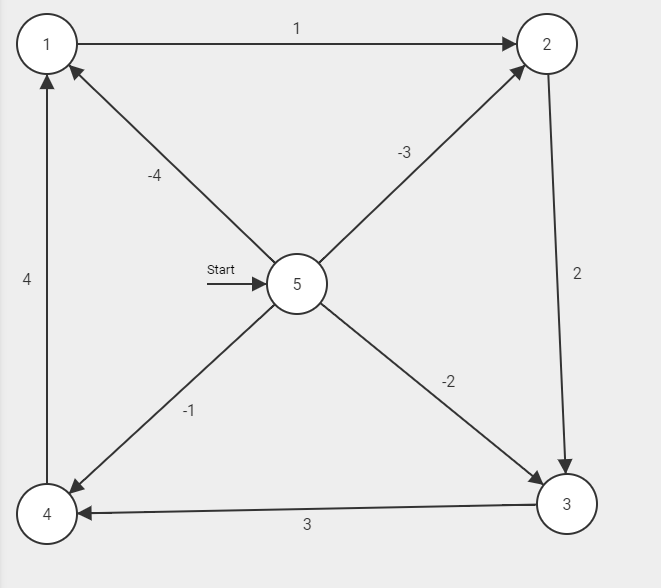
\includegraphics[width=0.9\linewidth]{02.png}
\label{fig:name}
\end{figure}

\section{Aufagbe 2}
Wenn unser counter auf -1 rennt müssen wir knoten finden 
den wir noch nie benutzt haben, dazu könnten wir einfach 
noch eine zweite Liste anlegen die am anfange alle
Elemente aus V enthält und wenn ein Knoten besucht 
wird wird dieser knoten aus der zweiten liste entfernt.

\section{Aufgabe 3}
\end{document}